\chapter{Guidelines}\label{chapter:guidelines}
\section{Context}\label{section:guidelines/context}
The major objective of the research is to devise some guidelines so that the task of approaching any complex problem domain using microservices becomes easier. On the way to that, a few research questions related to various crucial topics on microservices emerged. The research questions were taken as stepping stones for discovering guidelines. The topics are already covered in previous chapters. 
\\
At first, the concept related to granularity of microservices is studied in detail in chapter \ref{chapter:granularity}. In this chapter, the semantic meaning of size along with various dimensions defining granularity are discussed. Finally, various principles to help finding the optimum size for microservices are listed.
\\
Secondly, other quality attributes to be considered when designing good microservices were listed in chapter \ref{chapter:quality_of_service}. The quality metrices to determine each of these quality attributes are also mentioned. The various quality metrices lead to a limited list of basic metrices. Finally, various principles to qualify good services along with the way the quality attributes affect each other are recorded.
\\
Next, the ways to decompose problem domain in order to identify microservices are discussed in chapters \ref{chapter:service_candidate}, \ref{chapter:selection_by_use_case} and \ref{chapter:domain_driven_design}. The methods discussed are using domain driven design and use case refactoring. The steps involved in each method are described along with an example.
\\
Till then answers related to granularity , quality attributes and process of identifying microservices are derived from literature. In chapter \ref{chapter:hybris_architecture} attempt is made to find answeres from industry experience by studying the architecture at Hybris and conducting various interviews. With the knowledge, series of steps are shown to better visualize the process of breaking down problem domain into microservices.
\\
Finally, the challenges which come up while implementing microservices architecture are discussed in chapter \ref{chapter:challanges_of_microservices_architecture}. In this chapter, various ways to tackle these problems are described.

\section{Process to Microservices}\label{section:guidelines/process_to_microservices}
As shown in the figure \ref{fig:guidelines/chapter_nine_process}, the implementation of microservices consists of two major parts, understanding each part is crucial in order to follow microservice architecture.
\begin{enumerate}
\item \textbf{modeling microservices} \\
The core of the microservices architecture is problem domain and understanding it. Modeling microservices divides the problem domain into various components considering various internal quality attributes such as coupling, cohesion etc. The knowledge regarding quality attributes acts as an input when choosing the efficient process for identifying microservices from problem domain.
\item \textbf{operating the microservices artifacts in production environment} \\
The way microservices are designed to satisfy various external quality attributes such as scalability, resilience etc. However, it also introduces critical challenges. It is not entirely possible to get the advantages from microservice architecture unless these challenges are identified and tackled appropriately. In order to achieve that, certain implementation and operational practices of microservices need to be followed.
\end{enumerate}
\begin{figure}[H]
\begin{center}
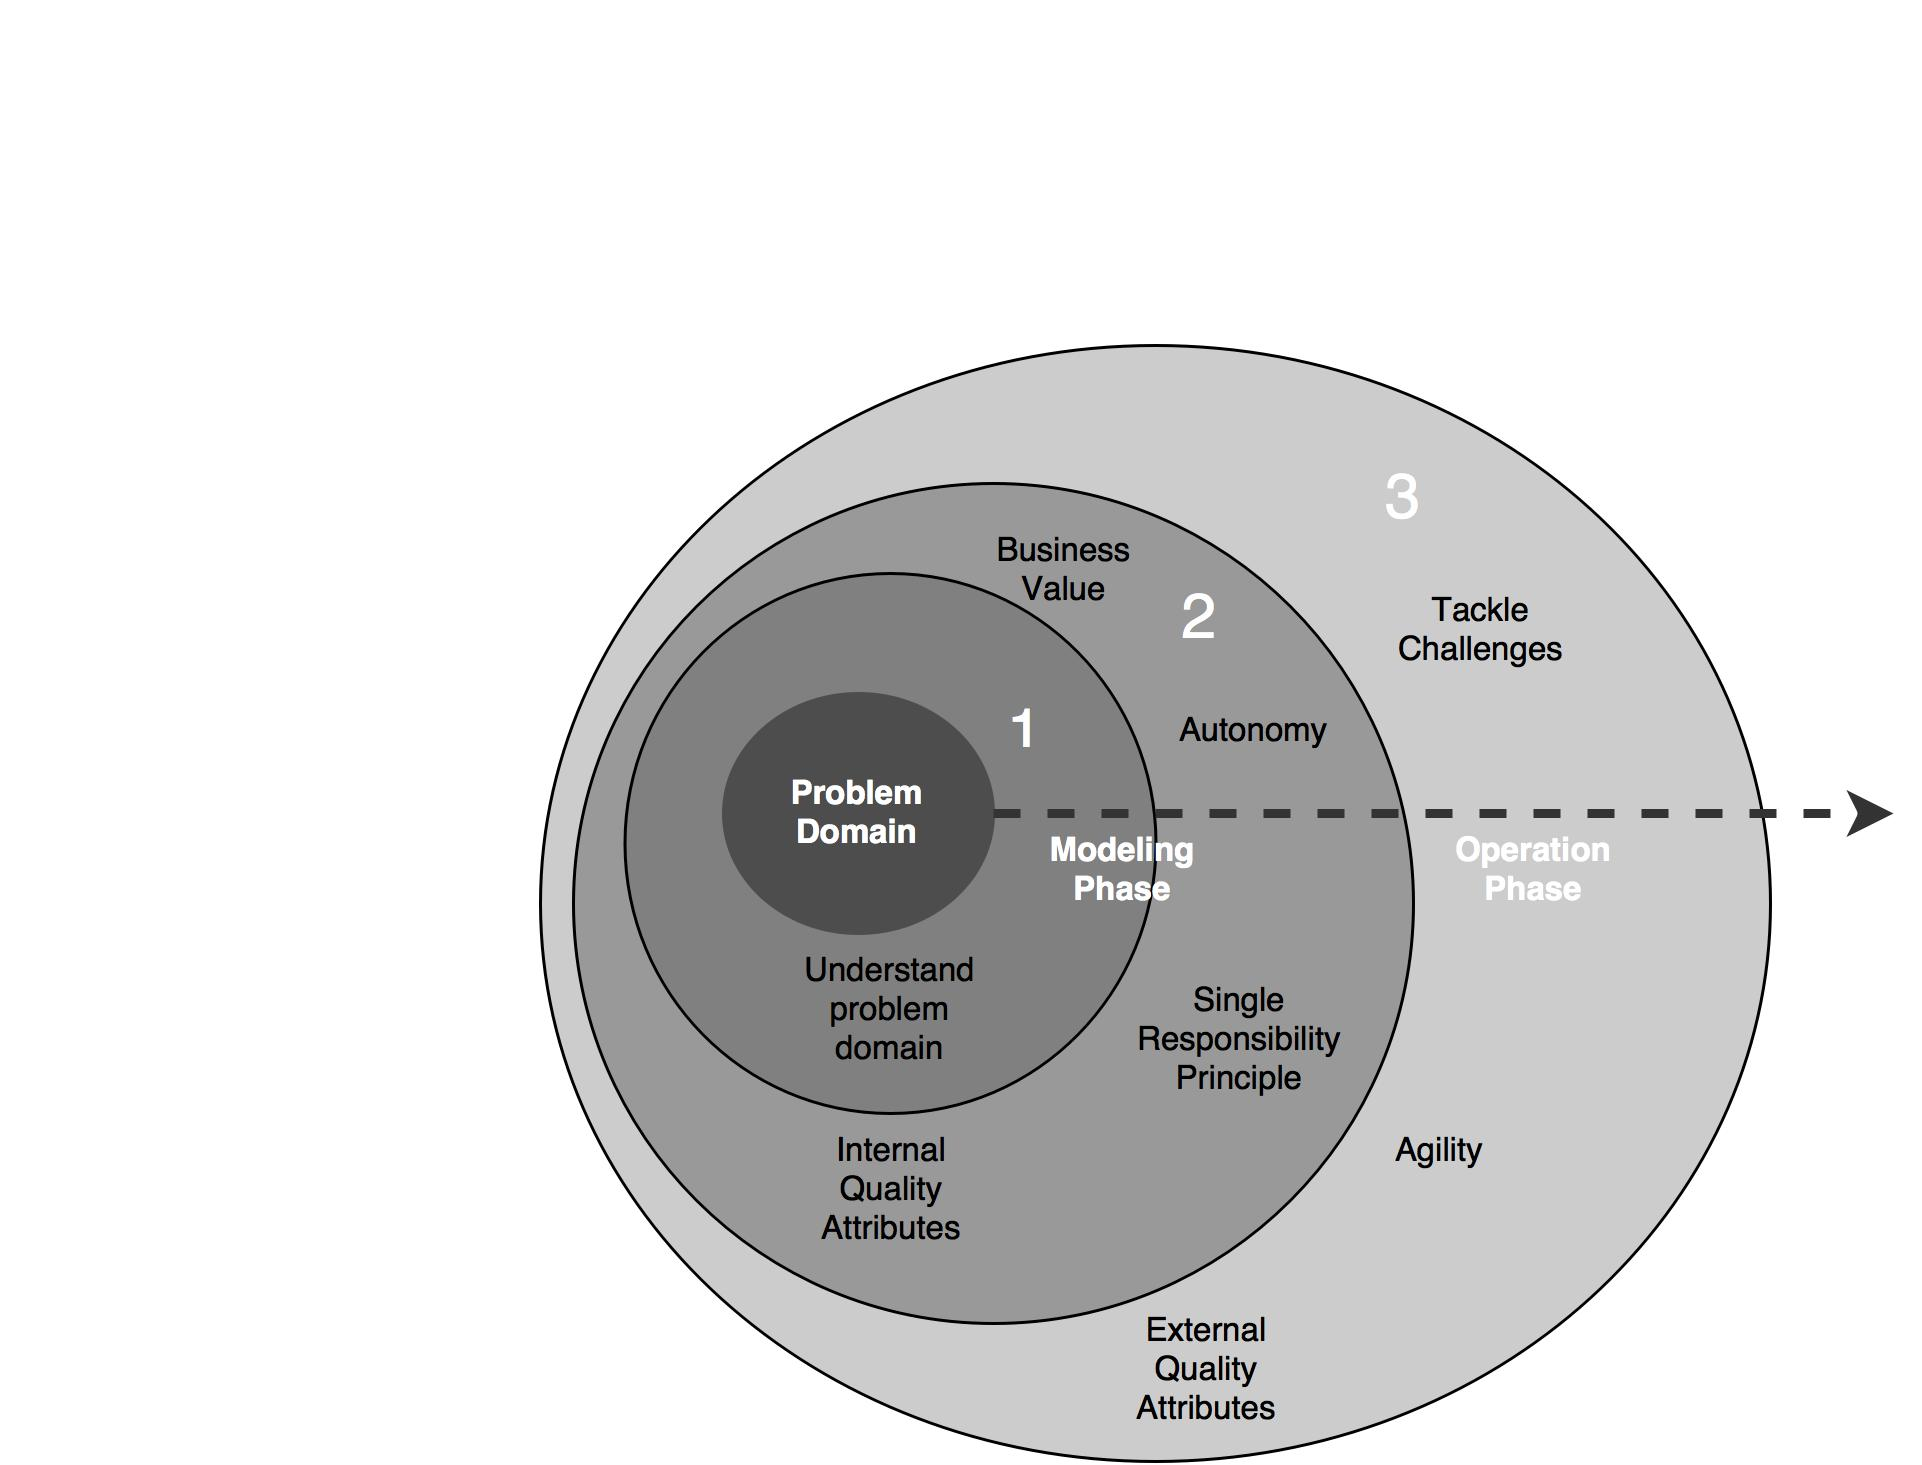
\includegraphics[width=0.7\textwidth]{figures/chapter_nine_process}
\caption{Process to microservice architecture}
\label{fig:guidelines/chapter_nine_process}
\end{center}
\end{figure}
\\
The microservices architecture follows a process which guides from understanding the problem domain, identifying modular components considering various attributes to implementing and operating the components to satisfy various external quality attributes. It is interesting find how process, principles and guidelines are related. A process is based upon some basic principles whereas principles helps to define guidelines based upon some specific requiement and environment. So, in order to understand the process of implementing microservices, it can be helpful to look into some broad basic principles.

\section{Principles}\label{section:guidelines/principles}
In this section, based upon the research findings as discussed in previous chapters, various principles are presented in order to tackle modeling microservices as well as operating them in release environment. \cite{Newman:2015aa}
\begin{enumerate}
\item \textbf{Correct Granularity} \\
The dimension of granularity for microservice is given by functionality it performs, data it handles and business value it provides. \ref{section:granularity/dimensions} These dimensions make it pretty obvious how to make the size of a service as low as possible. However, the notion of correct granularity is rather important and should be only focus instead of attempting to make the size lowest possible.\ref{section:granularity/principles} There are various factors which act together and tailor the size of microservice.
\begin{enumerate}
\item One of the factors is \textbf{\acrshort{SRP}}, which influence the functionalities and data handled by microservices to make it as small as possible. \acrshort{SRP} encourages to focus on small set of cohesive tasks which change for same reason. \cite{Stine:2014aa} \cite{Newman:2015aa} The influence of \acrshort{SRP} on is also verified by the result of interview which is compiled in section \ref{section:hybris_architecture/interview/interview_compilation}.
\item Another important factor is \textbf{autonomy}. According to S. Newman, a microservice should be able to be deployed and updated independently. \cite{Newman:2015aa} Without any surprise, autonomy is an important quality attribute of microservice and is evaluated as the degree of control upon operations to act on its business entities only. \ref{section:quality_of_service/quality_metrics/autonomy} As discussed in section \ref{section:granularity/principles}, a microservice should provide transaction integrity such that it is big enough to support activities which fall under one transaction. So, autonomy tends to limit the scope of functionality and data such that the service is self-contained, self-controlling and can be self-governed.\cite{Ma:2007aa}
\item The act of realizing the size of microservices as small as possible comes with a price. As the functionality of microservice is squeezed, the number of microservices needed for any application increases. The task of deploying, provisioning and governing these microservices can be challenging. So, as stated in the principles defined in section  \ref{principle:granularity/IT_infrastructure},  the decision regarding the size of service should be rational based upon the current \textbf{infrastructure and operational capability} to handle such large number of small microservices. It is further supported by the response of interview compilation \ref{section:hybris_architecture/interview/interview_compilation}
\item Finally, the size of microservices according to functionality and data should also relate to ultimate \textbf{business value} and should be coincide with the business goal. It is evident from the response of interview compiled in \ref{section:hybris_architecture/interview/interview_compilation}. Also, business value being an important dimension of granularity of microservice according to section \ref{section:granularity/dimensions}, should be examined before choosing the functionality being performed by a service.\\
So, while deciding about the size of microservice the mentioned factors should be well considered.

\item \textbf{Consider quality attributes as early as possible} \\
The internal quality attributes such as coupling, cohesion, autonomy etc should be controlled as early as possible during modeling and development phases. Taking care of the internal qualities will eventually help to control the external qualities of the microservices in release such as reusability, reliability, resilience etc. The table \ref{tab:quality_of_service/quality_attributes/basic_quality_metrics} which identifies various attributes in terms of basic metrices can be helpful. For one thing that the metrices such as scope of opertions, number of operations used in the basic metrices table are completely in disposal of the developers and teams of microservices. Secondly, it helps to identify the relationship among them as shown in table \ref{tab:quality_of_service/quality_attributes/quality_attributes_relationship} which assists in managing trade offs needed.

\item \textbf{Understand the problem domain}\\
As discussed in chapters , problem domain can be analyzed using either usecase modeling or domain driven design. \\
Using usecase can break down the problem domain into level of abstractions, each abstraction representing lower scope of functionality. The graphical approach used in usecase can be an effective approach in brainstorming and exploring the problem domain to find new usecases.\\
Another popular approach is using domain driven design to explore problem domain. The overal process looks natural and straight forward which focus on dividing the complex domain into manageable subdomains and further into modular autonomous components. Furthermore, it gives emphasis on using ubiquitous language to find modules and define their boundaries. The chapter provides important guidelines as well as hints on ubiquitous language and to find bounded contexts.\\
Although the graphical approach provided by usecases are wellsuited to experience so can be faster, but they tend to focus only on \acrshort{SRP} and scope of functionality. Following the process may likely lose grip on very important quality attribute of microservices which is autonomy.\\
Domain driven design on the other hand, with its approach of using ubiquitous language focus on autonomy and by dividing the problem domain into smaller manageable components also focus on autonomy. Although the whole proces seems natural, getting the boundary right is complex process. A clear understanding of the problem domain is necessary to get the bounded context right. So, it can be an iterative process starting at bigger boundaries at first and then down to smaller modular boundaries in several iterations.\\
The knowledge and practice of both usecase modeling and domain driven desing can be helpful. Depending upon the complexity of the problem domain and experience with it, any of them or combination of them can be used to understand the problem domain well.

\item \textbf{culture of automation}\\
With such a large number of small services, the task of managing and operating them manually can become impossible. There are three specific areas where automation can serve greatly.
\begin{enumerate}
\item Automated Continuous Delivery can help building and deploying microservices frequently with consistency. Maintaining continuous integration and delivery pipeline can make sure that any new changes is consistent to old system and can be put into release in a matter of few button presses.
\item Automated Testing is another important area to be serious when there are large number of microservices and again large number of changes in the backlog. Without automated testing in sync with delivery pipeline, it can be hard to have confidence of deploying changes to release environment without breaking existing functionalities.
\item Infrastructure Automation and provisioning should not be neglected, especially when there can be different technology stack in different microservices and different infrastructure environments. \acrshort{PAAS} such as CloudFoundry can be helpful to deployment and provision easily whereas various configuration management tools such as Puppet, chef etc can assist to manage different technology stacks.
\end{enumerate}
\item \textbf{hide internal implementation}\\
Collaboration among microservices is essential however high coupling by over exposing inter details should be avoided to save autonomy.
\begin{enumerate}
\item The first on the checklist is to model the \acrshort{API}s in right way. Rather than breaking the application into technological aspects, the problem domain should be clearly understood to discover clear boundaries and so should be modeled around business domains. The concept of bounded context can be a way to define clear \acrshort{API}s reducing unnecessary coupling.
\item The \acrshort{API}s should be technology agnostic, which means that the technology used for collaborating between \acrshort{API}s should not guide the implementation of them. Using \acrshort{REST} and some form of \acrshort{RPC} can help to mitigate them.
\item In microservices, database also an integral part of internal implementation. Already mentioned in section \ref{section:challanges_of_microservices_architecture/integration/shared_database}, sharing database will tightly couple microservices as it exposes internal data structure details. In order to mitigate that each microservice should atleast have its own private tables or schema per each service or at most separate database server.
\item Additionally, in order to maintain loose coupling, the integration technology should be well thought. As already discussed in section \ref{section:challanges_of_microservices_architecture/integration/inter_service_communication}, if business requirement allows, asynchronous communication styles such as publish/subscribe, notification, request/async response should be chosen over synchronous request/response.
\end{enumerate}
\item decentralize
\item deploy independently
\item consumer first
\item isolate failures
\item highly observable
\end{enumerate}